\documentclass[../mn-notatki.tex]{subfiles}

\begin{document}

\section{Automatyczne różniczkowanie}

\subsection{Metoda propagacji w przód}


\subsubsection{Funkcja jednej zmiennej}
\begin{tcolorbox}
\[
\vec{x} = (x, 1, 0, \ldots) ~~~~~~~~ \vec{c} = (c, 0, 0, \ldots)
\]
\[
\vec{u} = (u, u', u'', \ldots)
\]
\[
\vec{g}(\vec{u}) = (u, u', u'', \ldots)
= (g(u), u'g'(u), u''g'(u) + (u')^2 g''(u), \ldots)
\]
\end{tcolorbox}

\begin{tcolorbox}
\textbf{Operacje na dżetach postaci $(u, u')$}
    $$(u,u') + (v,v') = (u + v, u' + v')$$
    $$(u,u') - (v,v') = (u - v, u' - v')$$
    $$(u,u') \cdot (v,v') = (u \cdot v, u \cdot v' + u' \cdot v)$$
    $$\frac{(u,u')}{(v,v')} = \left(\frac{u}{v}, \frac{u' - \frac{u}{v}\cdot v'}{v}\right)$$
    $$\sin(u,u') = (\sin u, \cos u \cdot u')$$
    $$\cos(u,u') = (\cos u, -\sin u \cdot u')$$
    $$e^{(u,u')} = (e^u, u' \cdot e^u)$$
    $$\ln(u,u') = \left(\ln u, \frac{u'}{u}\right)$$
\end{tcolorbox}

\subsubsection{Pochodne kierunkowe}
\begin{tcolorbox}
\[
f: \mathbb{R}^n \rightarrow \mathbb{R}, x, u \in \mathbb{R}^n:
g(t) = f(x + t \cdot u)
\]
\[
g'(t) = u \cdot \nabla f(t \cdot u + x) \Rightarrow g'(0) = u \cdot \nabla f(x)
\]
\[
x = ((x_1, 0), (x_2, 0), \ldots, (x_n, 0))
\]
\[
u = ((u_1, 0), (u_2, 0), \ldots, (u_n, 0))
\]
\[
t = (0,1)
\]
\end{tcolorbox}
Redukujemy problem obliczenia $\nabla_u f(x)$ do obliczenia pochodnej funkcji
jednej zmiennej.
% Poniważ chcemy policzyć pochodną w punkcie $t = 0$, zmienna $t$ zostanie
% zastąpiona parą $(0,1)$, natomiast $x = ((x_1, 0), (x_2, 0), \ldots, (x_n, 0))$,
% $u = ((u_1, 0), (u_2, 0), \ldots, (u_n, 0))$.

\subsubsection{Gradient}
Aby obliczyć pochodne cząstkowe funkcji $f$ wystarczy obliczyć
$\nabla_{e_i}f(x)$,
% ($i = 1, \ldots, n$),
gdzie $e_i$ to wektor z bazy $\mathbb{R}^n$.

\begin{tcolorbox}
\[
\vec{x} = (x, 1, 0, 0, \ldots) ~~~~~~~~ \vec{y} = (y, 0, 1, 0, \ldots) ~~~~~~~~ \vec{c} = (c, 0, 0, 0, \ldots)
\]
% \[
% \vec{u} = (u, u', u'', \ldots)
% \]
\[
\vec{f}(\vec{x}) = \left(f(x), \frac{\partial f}{\partial x}, \frac{\partial f}{\partial y}, \ldots \right)
% = (g(u), u'g'(u), u''g'(u) + (u')^2 g''(u), \ldots)
\]
\end{tcolorbox}

\begin{tcolorbox}
\textbf{Operacje na dżetach $m+1$ wymiarowych wektorów}
    $$(u,u_1,\ldots, u_m) + (v,v_1,\ldots, v_m) = (u + v, u_1 + v_1, \ldots, u_m + v_m)$$
    $$(u,u_1,\ldots, u_m) - (v,v_1,\ldots, v_m) = (u - v, u_1 - v_1, \ldots, u_m - v_m)$$
    $$(u,u_1,\ldots, u_m) \cdot (v,v_1,\ldots, v_m) = (u \cdot v, u \cdot v_1 + u_1 \cdot v, \ldots, u \cdot v_m + u_m \cdot v)$$
    $$\frac{(u,u_1,\ldots, u_m)}{(v,v_1,\ldots, v_m)} = \left(\frac{u}{v}, \frac{u_1 - \frac{u}{v}\cdot v_1}{v}, \ldots, \frac{u_m - \frac{u}{v}\cdot v_m}{v}\right)$$
    $$\sin(u,u_1,\ldots, u_m) = \text{zostawiam jako ćwiczenie dla czytelnika}$$
    $$\cos(u,u_1,\ldots, u_m) = \ldots$$
    $$e^{(u,u_1,\ldots, u_m)} = \ldots$$
\end{tcolorbox}

\subsection{Metoda akumulacji wstecz}
\begin{tcolorbox}
\[
\bar{v_i} = \frac{\partial f}{\partial v_i}
\]
\end{tcolorbox}
\begin{tcolorbox}
% \textbf{Przykład}
\[
f(x, y, z) = \frac{(x+y)(y+z) - 1}{xyz + 2}, x = (1, 3, 1)
\]
\end{tcolorbox}

% {"nodes":[{"x":95,"y":147,"text":"x","isAcceptState":false},{"x":278,"y":147,"text":"y","isAcceptState":false},{"x":463,"y":137,"text":"z","isAcceptState":false},{"x":95,"y":259,"text":"v_1 = x+y","isAcceptState":false},{"x":278,"y":259,"text":"v_2 = y+z","isAcceptState":false},{"x":555,"y":47,"text":"v_5=x\\cdot y","isAcceptState":false},{"x":182,"y":357,"text":"v_3 = v_1 \\cdot v_2","isAcceptState":false},{"x":182,"y":453,"text":"v_4 = v_3 - 1","isAcceptState":false},{"x":51,"y":357,"text":"1","isAcceptState":false},{"x":463,"y":259,"text":"v_6 = v_5 \\cdot z","isAcceptState":false},{"x":463,"y":357,"text":"v_7 = v_6 + 2","isAcceptState":false},{"x":621,"y":259,"text":"2","isAcceptState":false},{"x":356,"y":478,"text":"v_8 = \\frac{v_4}{v_7}","isAcceptState":false}],"links":[{"type":"Link","nodeA":0,"nodeB":3,"text":"","lineAngleAdjust":0,"parallelPart":0.5,"perpendicularPart":0},{"type":"Link","nodeA":1,"nodeB":3,"text":"","lineAngleAdjust":0,"parallelPart":0.5,"perpendicularPart":0},{"type":"Link","nodeA":2,"nodeB":4,"text":"","lineAngleAdjust":0,"parallelPart":0.5,"perpendicularPart":0},{"type":"Link","nodeA":1,"nodeB":4,"text":"","lineAngleAdjust":0,"parallelPart":0.5,"perpendicularPart":0},{"type":"Link","nodeA":1,"nodeB":5,"text":"","lineAngleAdjust":0,"parallelPart":0.6183514164812233,"perpendicularPart":16.835435412500782},{"type":"Link","nodeA":0,"nodeB":5,"text":"","lineAngleAdjust":3.141592653589793,"parallelPart":0.6116425992779784,"perpendicularPart":-81.7004412097194},{"type":"Link","nodeA":2,"nodeB":9,"text":"","lineAngleAdjust":0,"parallelPart":0.5,"perpendicularPart":0},{"type":"Link","nodeA":5,"nodeB":9,"text":"","lineAngleAdjust":3.141592653589793,"parallelPart":0.3449670461354104,"perpendicularPart":-24.785623696029887},{"type":"Link","nodeA":3,"nodeB":6,"text":"","lineAngleAdjust":0,"parallelPart":0.5,"perpendicularPart":0},{"type":"Link","nodeA":4,"nodeB":6,"text":"","lineAngleAdjust":0,"parallelPart":0.5,"perpendicularPart":0},{"type":"Link","nodeA":6,"nodeB":7,"text":"","lineAngleAdjust":0,"parallelPart":0.5,"perpendicularPart":0},{"type":"Link","nodeA":8,"nodeB":7,"text":"","lineAngleAdjust":0,"parallelPart":0.5,"perpendicularPart":0},{"type":"Link","nodeA":7,"nodeB":12,"text":"","lineAngleAdjust":3.141592653589793,"parallelPart":0.6018018018018018,"perpendicularPart":-34.52378733412503},{"type":"Link","nodeA":10,"nodeB":12,"text":"","lineAngleAdjust":3.141592653589793,"parallelPart":0.4864439927905818,"perpendicularPart":0},{"type":"Link","nodeA":11,"nodeB":10,"text":"","lineAngleAdjust":0,"parallelPart":0.5,"perpendicularPart":0},{"type":"Link","nodeA":9,"nodeB":10,"text":"","lineAngleAdjust":0,"parallelPart":0.5,"perpendicularPart":0}]}

\begin{center}
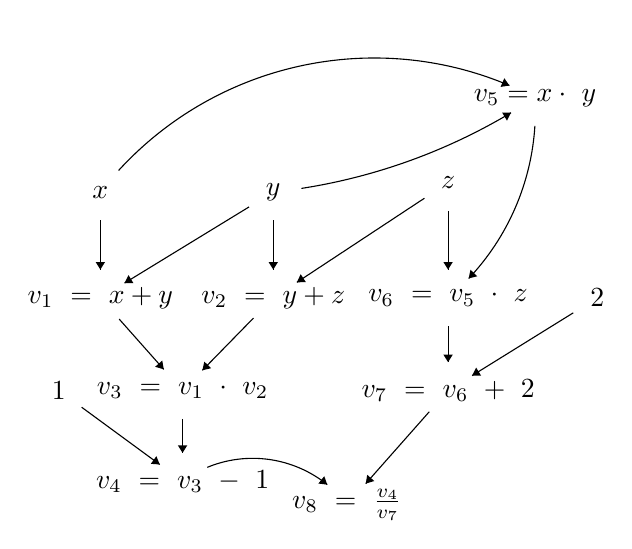
\begin{tikzpicture}[scale=0.12]
\tikzstyle{every node}+=[inner sep=0pt]
% \draw [black] (9.5,-14.7) circle (3);
\draw (9.5,-14.7) node {$x$};
% \draw [black] (27.8,-14.7) circle (3);
\draw (27.8,-14.7) node {$y$};
% \draw [black] (46.3,-13.7) circle (3);
\draw (46.3,-13.7) node {$z$};
% \draw [black] (9.5,-25.9) circle (3);
\draw (9.5,-25.9) node {$v_1\mbox{ }=\mbox{ }x+y$};
% \draw [black] (27.8,-25.9) circle (3);
\draw (27.8,-25.9) node {$v_2\mbox{ }=\mbox{ }y+z$};
% \draw [black] (55.5,-4.7) circle (3);
\draw (55.5,-4.7) node {$v_5=x\cdot\mbox{ }y$};
% \draw [black] (18.2,-35.7) circle (3);
\draw (18.2,-35.7) node {$v_3\mbox{ }=\mbox{ }v_1\mbox{ }\cdot\mbox{ }v_2$};
% \draw [black] (18.2,-45.3) circle (3);
\draw (18.2,-45.3) node {$v_4\mbox{ }=\mbox{ }v_3\mbox{ }-\mbox{ }1$};
% \draw [black] (5.1,-35.7) circle (3);
\draw (5.1,-35.7) node {$1$};
% \draw [black] (46.3,-25.9) circle (3);
\draw (46.3,-25.9) node {$v_6\mbox{ }=\mbox{ }v_5\mbox{ }\cdot\mbox{ }z$};
% \draw [black] (46.3,-35.7) circle (3);
\draw (46.3,-35.7) node {$v_7\mbox{ }=\mbox{ }v_6\mbox{ }+\mbox{ }2$};
% \draw [black] (62.1,-25.9) circle (3);
\draw (62.1,-25.9) node {$2$};
% \draw [black] (35.6,-47.8) circle (3);
\draw (35.6,-47.8) node {$v_8\mbox{ }=\mbox{ }\frac{v_4}{v_7}$};
\draw [black] (9.5,-17.7) -- (9.5,-22.9);
\fill [black] (9.5,-22.9) -- (10,-22.1) -- (9,-22.1);
\draw [black] (25.24,-16.27) -- (12.06,-24.33);
\fill [black] (12.06,-24.33) -- (13,-24.34) -- (12.48,-23.49);
\draw [black] (43.8,-15.35) -- (30.3,-24.25);
\fill [black] (30.3,-24.25) -- (31.25,-24.23) -- (30.7,-23.39);
\draw [black] (27.8,-17.7) -- (27.8,-22.9);
\fill [black] (27.8,-22.9) -- (28.3,-22.1) -- (27.3,-22.1);
\draw [black] (52.963,-6.301) arc (-59.13361:-81.16613:61.727);
\fill [black] (52.96,-6.3) -- (52.02,-6.28) -- (52.53,-7.14);
\draw [black] (11.434,-12.408) arc (137.49957:67.02998:36.678);
\fill [black] (52.79,-3.42) -- (52.25,-2.65) -- (51.86,-3.57);
\draw [black] (46.3,-16.7) -- (46.3,-22.9);
\fill [black] (46.3,-22.9) -- (46.8,-22.1) -- (45.8,-22.1);
\draw [black] (55.489,-7.698) arc (-3.54341:-43.37463:25.834);
\fill [black] (48.48,-23.84) -- (49.39,-23.61) -- (48.67,-22.92);
\draw [black] (11.49,-28.14) -- (16.21,-33.46);
\fill [black] (16.21,-33.46) -- (16.05,-32.53) -- (15.3,-33.19);
\draw [black] (25.7,-28.04) -- (20.3,-33.56);
\fill [black] (20.3,-33.56) -- (21.22,-33.34) -- (20.5,-32.64);
\draw [black] (18.2,-38.7) -- (18.2,-42.3);
\fill [black] (18.2,-42.3) -- (18.7,-41.5) -- (17.7,-41.5);
\draw [black] (7.52,-37.47) -- (15.78,-43.53);
\fill [black] (15.78,-43.53) -- (15.43,-42.65) -- (14.84,-43.46);
\draw [black] (20.81,-43.834) arc (112.48571:51.1619:12.579);
\fill [black] (33.51,-45.66) -- (33.2,-44.77) -- (32.57,-45.55);
\draw [black] (44.31,-37.95) -- (37.59,-45.55);
\fill [black] (37.59,-45.55) -- (38.49,-45.28) -- (37.74,-44.62);
\draw [black] (59.55,-27.48) -- (48.85,-34.12);
\fill [black] (48.85,-34.12) -- (49.79,-34.12) -- (49.27,-33.27);
\draw [black] (46.3,-28.9) -- (46.3,-32.7);
\fill [black] (46.3,-32.7) -- (46.8,-31.9) -- (45.8,-31.9);
\end{tikzpicture}
\end{center}

\begin{minipage}{.5\textwidth}
\begin{center}
        $v_1 = 4$\\
        $v_2 = 4$\\
        $v_3 = 16$\\
        $v_4 = 16$\\
        $v_5 = 3$\\
        $v_6 = 3$\\
        $v_7 = 5$\\
        $f = v_8 = 3$
\end{center}
\end{minipage}%
\begin{minipage}{.5\textwidth}
    % \begin{gather*}
\begin{center}
        $\bar{v_8} = 1$\\
        $\bar{v_7} = \frac{\partial f}{\partial v_8} \cdot \frac{\partial v_8}{\partial v_7} = -\frac{3}{5}$\\
        $\bar{v_6} = \frac{\partial f}{\partial v_7} \cdot \frac{\partial v_7}{\partial v_6} = -\frac{3}{5}$\\
        $\bar{v_5} = \frac{\partial f}{\partial v_6} \cdot \frac{\partial v_6}{\partial v_5} = -\frac{3}{5}$\\
        $\bar{v_4} = \frac{\partial f}{\partial v_8} \cdot \frac{\partial v_8}{\partial v_4} = \frac{1}{5}$\\
        $\bar{v_3} = \frac{\partial f}{\partial v_4} \cdot \frac{\partial v_4}{\partial v_3} = \frac{1}{5}$\\
        $\bar{v_2} = \frac{\partial f}{\partial v_3} \cdot \frac{\partial v_3}{\partial v_1} = \frac{4}{5}$\\
        $\bar{v_1} = \frac{\partial f}{\partial v_3} \cdot \frac{\partial v_3}{\partial v_2} = \frac{4}{5}$
\end{center}
    % \end{gather*}
\end{minipage}
\[
\frac{\partial f}{\partial x}(1,3,1) = \bar{v_1} \frac{\partial f}{\partial x}
+ \bar{v_5}\frac{\partial f}{\partial x} = -1
\]

\subsection{Automatyczne różniczkowanie z wykorzystaniem szeregu Taylora}
\begin{tcolorbox}
\[
f_k = \frac{f^{(k)}(x_0)}{k!}
\]
\[
\vec{f} = (f_0, f_1, f_2, \ldots)
\]
% \[
% \vec{f}(\vec{x}) = \left(f(x), \frac{\partial f}{\partial x}, \frac{\partial f}{\partial y}, \ldots \right)
% % = (g(u), u'g'(u), u''g'(u) + (u')^2 g''(u), \ldots)
% \]
\end{tcolorbox}

\begin{tcolorbox}
\textbf{Arytmetyka}
    $$(f + g)_k  = f_k + g_k$$
    $$(f - g)_k  = f_k - g_k$$
    $$(f \cdot g)_k  = \sum_{i=0}^{k} f_i \cdot g_{k-i}$$
    $$\left(\frac{f}{g}\right)_k  = \frac{1}{g_0} \cdot \left( f_k - \sum_{i=0}^{k-1} \frac{f}{g}_{i} \cdot g_{k-i} \right)$$
    $$(\sin g)_k = \frac{1}{k} \cdot \sum_{i=1}^{k} i \cdot g_i \cdot (\cos g)_{k-1}$$
    $$(\cos g)_k = -\frac{1}{k} \cdot \sum_{i=1}^{k} i \cdot g_i \cdot (\sin g)_{k-1}$$
    $$
    (e^g)_k =
    \begin{cases}
    e^{g_0}, ~~~~~~ k = 0\\
    \frac{1}{k} \cdot \sum_{i=1}^{k} i \cdot g_i \cdot \left(e_g\right)_{k-1},~~~~~~ k >0
    \end{cases}
    $$
    $$
    (g^a)_k =  \frac{1}{g_0} \cdot \left( \sum_{i=1}^{k} \frac{a\cdot i}{k}g_i \cdot (g^a)_{k-i}- \sum_{i=1}^{k-1} \frac{i}{k} (g^a)_i \cdot g_{k-i}\right)
    $$
\end{tcolorbox}

\pagebreak
\end{document}
